\documentclass[11pt]{amsart}
\usepackage[margin=1in]{geometry}
\usepackage{amsmath,amssymb,amsthm,mathtools}
\usepackage{graphicx}
\usepackage{booktabs}
\usepackage{enumitem}
\usepackage{microtype}
\usepackage{xcolor}
\usepackage[colorlinks=true,linkcolor=blue!50!black,citecolor=green!40!black,urlcolor=blue!50!black]{hyperref}

\newcommand{\repourl}{https://github.com/jackelinemontalvo221-cyber/lpk-conjecture-n6}

\newtheorem{theorem}{Theorem}[section]
\newtheorem{proposition}[theorem]{Proposition}
\newtheorem{lemma}[theorem]{Lemma}
\newtheorem{corollary}[theorem]{Corollary}
\theoremstyle{definition}
\newtheorem{definition}[theorem]{Definition}
\theoremstyle{remark}
\newtheorem{remark}[theorem]{Remark}

\newcommand{\C}{\mathbb{C}}
\newcommand{\R}{\mathbb{R}}
\newcommand{\Z}{\mathbb{Z}}
\newcommand{\Q}{\mathbb{Q}}
\newcommand{\cD}{\mathcal{D}}
\newcommand{\conv}{\operatorname{conv}}
\newcommand{\cross}{\operatorname{cr}}
\newcommand{\dotp}{\operatorname{dt}}
\renewcommand{\Im}{\operatorname{Im}}
\renewcommand{\Re}{\operatorname{Re}}
\newcommand{\PM}{\mathrm{PM}}
\newcommand{\Pn}{\mathrm{P}_{90}}
\newcommand{\sq}{\tfrac{\sqrt3}{2}}

\title[Convexly independent eigenvectors of $6\times6$ doubly stochastic matrices]{Eigenvalues of $6\times 6$ doubly stochastic matrices\\ with convexly independent eigenvectors}
\author{Hengrui Zhu}
\address{Yuquan College, University of Chinese Academy of Sciences}
\date{October 2026}
\subjclass[2020]{15B51, 15A18, 52A10, 65G30}
\keywords{doubly stochastic matrix, Perfect--Mirsky conjecture, Karpelevi\v{c} region, convexly independent, computer-assisted proof, interval arithmetic}

\begin{document}

\begin{abstract}
Levick, Pereira and Kribs conjectured that if an eigenvalue $\lambda$ of an $n\times n$ doubly stochastic matrix has an eigenvector whose entries are convexly independent, then $\lambda$ lies in the Perfect--Mirsky region $\bigcup_{k\le n}\Pi_k$, where $\Pi_k$ is the convex hull of the $k$-th roots of unity. We prove the stronger inclusion $\lambda\in\Pi_6$ for $n=6$; consequently, the eigenvalues of $6\times6$ doubly stochastic matrices that admit a convexly independent eigenvector form exactly the regular hexagon $\Pi_6$. The proof splits according to $\arg\lambda$. The sector $\lvert\arg\lambda\rvert\le\pi/3$ follows from a classical bound of Dmitriev and Dynkin. For $\lvert\arg\lambda\rvert\ge2\pi/3$ we use that the convex hull of the $3$-element subset sums of the eigenvector is centrally symmetric, which reduces the problem to real $3\times3$ matrices whose columns have $\ell^1$-norm at most $1$. The middle sector reduces to a statement about hexagons formed by two interleaved triangles with centroid at the origin. This statement is sharp along a two-parameter family of hexagons; we prove it by combining three exact ``potential'' lemmas with a branch-and-bound computation whose $53{,}093$ boxes are verified in ball arithmetic. Bouthat, Mashreghi and Morneau-Guérin have announced, in talks, the inclusion $\lambda\in\Pi_n$ for all $n$; the argument given here for $n=6$ is independent of theirs.
\end{abstract}

\maketitle

\section{Introduction}

A real square matrix is \emph{doubly stochastic} if its entries are nonnegative and all its row and column sums are equal to $1$. Let $\cD_n$ denote the set of $n\times n$ doubly stochastic matrices and
\[
\omega_n=\{\lambda\in\C:\ \lambda \text{ is an eigenvalue of some } A\in\cD_n\}.
\]
For $k\ge1$ let $\Pi_k=\conv\{e^{2\pi ij/k}:0\le j<k\}$ be the convex hull of the $k$-th roots of unity (so $\Pi_1=\{1\}$ and $\Pi_2=[-1,1]$), and let $\PM_n=\bigcup_{k=1}^n\Pi_k$. Taking convex combinations of the powers of the permutation matrix of a $k$-cycle ($k\le n$) shows that $\Pi_k\subseteq\omega_n$, so $\PM_n\subseteq\omega_n$, and Perfect and Mirsky \cite{PM65} conjectured that $\omega_n=\PM_n$. The conjecture holds for $n\le3$ \cite{PM65} and for $n=4$ \cite{LPK15}; it fails for $n=5$ \cite{MR07} (see \cite{HJL} for a detailed computational study of the exceptional region); and it is open for every $n\ge6$. Harlev, Johnson and Lim \cite{HJL} formulate a conjecture on the boundary of $\omega_n$ and give computational evidence that, if it holds, then $\omega_n=\PM_n$ for $6\le n\le11$.

After settling the case $n=4$, Levick, Pereira and Kribs \cite{LPK15} proposed three conjectures. Conjectures~1 and~3 of \cite{LPK15} were disproved for all $n\ge5$ by Kim and Kim \cite{KK22}. Following \cite[Definition~2]{LPK15}, the entries of a vector $v\in\C^n$ are \emph{convexly independent} if no $v_i$ lies in the convex hull of the other entries; equivalently, $v_1,\dots,v_n$ are the $n$ vertices of a convex $n$-gon.

\begin{quote}
\textbf{Conjecture 2 of \cite{LPK15}.} Let $A\in\cD_n$ and let $\lambda$ be an eigenvalue of $A$. If the entries of an eigenvector corresponding to $\lambda$ are convexly independent, then $\lambda\in\PM_n$.
\end{quote}

Our main result settles this conjecture for $n=6$, in the stronger form $\lambda\in\Pi_6$.

\begin{theorem}\label{thm:main}
Let $A\in\cD_6$ and let $\lambda$ be an eigenvalue of $A$. If $\lambda$ has a right or a left eigenvector whose six entries are convexly independent, then $\lambda\in\Pi_6$.
\end{theorem}

The inclusion is sharp: if $P$ is the permutation matrix of a $6$-cycle, then $(\zeta^j)_{j=1}^6$ with $\zeta=e^{i\pi/3}$ is an eigenvector of every matrix $\sum_{l=0}^{5}c_lP^l$ ($c_l\ge0$, $\sum c_l=1$), its entries form a regular hexagon, and the corresponding eigenvalues fill $\Pi_6$. Hence the set of eigenvalues of matrices in $\cD_6$ admitting a convexly independent (left or right) eigenvector is exactly $\Pi_6$. Theorem~\ref{thm:main} also says where a counterexample to the Perfect--Mirsky conjecture for $n=6$ cannot come from:

\begin{corollary}\label{cor:pm}
If $\lambda\in\omega_6\setminus\PM_6$, then no left or right eigenvector of any $A\in\cD_6$ for the eigenvalue $\lambda$ has convexly independent entries.
\end{corollary}

\subsection*{Relation to the work of Bouthat, Mashreghi and Morneau-Guérin}
In two talks given in May 2026 \cite{Bou26,BMM26} (see also the poster \cite{BMM25}), Bouthat, Mashreghi and Morneau-Guérin announced a theorem stating that, for every $n$, an eigenvalue of an $n\times n$ doubly stochastic matrix with a convexly independent eigenvector lies in $\Pi_n$. Theorem~\ref{thm:main} is therefore the case $n=6$ of their announced result. To our knowledge their paper is not yet publicly available. As far as we can tell from the slides, their approach considers, in each direction, an eigenpair of maximal modulus with a convexly independent eigenvector $z$, and aims to show that the vector of midpoints $\bigl(\frac{z_1+z_2}{2},\dots,\frac{z_n+z_1}{2}\bigr)$ is again a maximal eigenvector; iterating, one reaches affinely regular polygons, on which $\lvert\lambda\rvert$ can be maximized directly. This maximality-preservation step is labelled as a conjecture in the slides of the ILAS talk \cite{BMM26} and in one version of the Delaware slides \cite{Bou26}; another version of the Delaware slides, the file currently attached to the r-libre record of that talk \cite{Bou26b}, labels it a proposition, without proof. We have not seen a written proof of this step. The proof given here follows a different route and does not depend on that step. It is specific to $n=6$, it uses only $\sum_iv_i=0$ and the inclusions $\lambda K_m(v)\subseteq K_m(v)$ for $m=1,2,3$, where $K_m(v)$ is the convex hull of the sums of $m$ entries of $v$ with distinct indices (Section~\ref{sec:prelim}), and part of it is computer-assisted.

\subsection*{Outline of the proof}
Let $Av=\lambda v$ with $\lambda\notin\R$, $\operatorname{Im}\lambda>0$, and assume that the entries of $v$ are convexly independent. For $1\le m\le 5$ let $K_m(v)$ be the convex hull of the sums $\sum_{i\in S}v_i$ over all $m$-element sets $S\subseteq\{1,\dots,6\}$. Then $\sum_iv_i=0$ and $\lambda K_m(v)\subseteq K_m(v)$ for every $m$ (Lemma~\ref{lem:Km}). We distinguish three sectors (Figure~\ref{fig:overview}).
\begin{enumerate}[leftmargin=2em]
\item $0<\arg\lambda\le\pi/3$. Since $\omega_6$ is contained in the Karpelevi\v{c} region $\Theta_6$ (the set of eigenvalues of $6\times6$ stochastic matrices), a classical bound of Dmitriev and Dynkin gives $\lambda\in\Pi_6$ (Theorem~\ref{thm:DD}). Convex independence is not needed here.
\item $2\pi/3\le\arg\lambda<\pi$. Because $n=6$ is even and $\sum_iv_i=0$, the polygon $K_3(v)$ is centrally symmetric, and under convex independence it is a hexagon. The inclusion $\lambda K_3(v)\subseteq K_3(v)$ then shows that $\lambda$ is an eigenvalue of a real $3\times3$ matrix whose columns have $\ell^1$-norm at most $1$, and such eigenvalues lie in $\Theta_6$. Applying the Dmitriev--Dynkin bound to $-\bar\lambda$ gives $\lambda\in\Pi_6$ (Proposition~\ref{prop:K3}). This is the analogue of the argument of \cite{LPK15} for $n=4$, where $K_2(v)$ is a parallelogram.
\item $\pi/3<\arg\lambda<2\pi/3$. Here $\lambda\in\Pi_6$ means $\operatorname{Im}\lambda\le\sqrt3/2$. The hexagon $H=K_2(v)$ has vertices $s_j=v_j+v_{j+1}$, and the triangles $s_1s_3s_5$ and $s_2s_4s_6$ both have centroid $0$. We show that every such hexagon contains a point $x\neq0$ with $\operatorname{Im}(s_j/x)\le\sqrt3/2$ for all $j$ (Proposition~\ref{prop:P90}, which we call $\Pn$); since $\lambda x\in H$, this forces $\operatorname{Im}\lambda\le\sqrt3/2$ (Lemma~\ref{lem:single}).
\end{enumerate}
Proposition $\Pn$ is the heart of the matter. It is sharp along a two-parameter family of hexagons (Remark~\ref{rem:sharp}), so it cannot be verified by a direct interval computation of its margin. We prove three exact lemmas (Section~\ref{sec:lemmas}), each of which produces a witness vertex provided one particular inequality holds, and we use a branch-and-bound computation in ball arithmetic to check that, everywhere in a compact $6$-dimensional box of parameters, one of finitely many such certificates applies (Section~\ref{sec:computer}).

\begin{figure}[t]
\centering
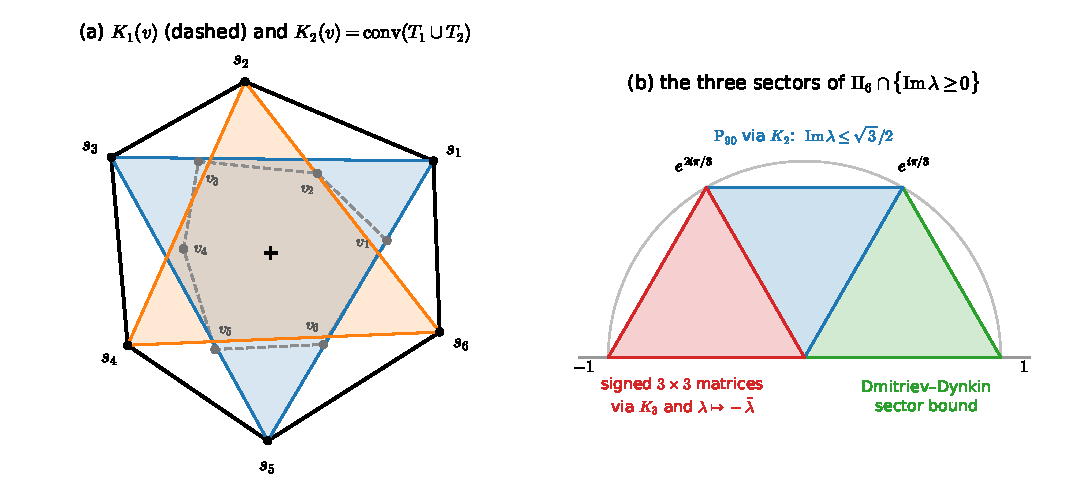
\includegraphics[width=\textwidth]{fig_overview.pdf}
\caption{(a) A convexly independent vector $v$ with $\sum_iv_i=0$; the hexagon $K_2(v)$ has the vertices $s_j=v_j+v_{j+1}$, and $T_1=s_1s_3s_5$, $T_2=s_2s_4s_6$ are triangles with centroid $0$. (b) The three sectors of the proof of Theorem~\ref{thm:main}: Theorem~\ref{thm:DD} for $\lvert\arg\lambda\rvert\le\pi/3$, Proposition~\ref{prop:P90} with Lemma~\ref{lem:single} for $\pi/3<\lvert\arg\lambda\rvert<2\pi/3$, and Proposition~\ref{prop:K3} for $\lvert\arg\lambda\rvert\ge2\pi/3$.}
\label{fig:overview}
\end{figure}

\subsection*{Notation}
For $a,b\in\C$ we write $\cross(a,b)=\operatorname{Im}(\bar ab)$ and $\dotp(a,b)=\operatorname{Re}(\bar ab)$ for the cross and dot products of $a,b$ viewed as vectors in $\R^2$. Throughout, $\zeta=e^{i\pi/3}$ and $\omega=\zeta^2=e^{2\pi i/3}$. Indices of vertices of hexagons are taken modulo $6$. For a compact convex set $H\subset\C$ we write $S(H)=\{\lambda\in\C:\lambda H\subseteq H\}$ and $h_H(\varphi)=\max_{z\in H}\Re(ze^{-i\varphi})$ for its support function.

\section{Preliminaries}\label{sec:prelim}

\subsection{Subset-sum polygons}
For $v\in\C^n$ and $1\le m\le n-1$ let
\[
K_m(v)=\conv\Bigl\{\sum_{i\in S}v_i:\ S\subseteq\{1,\dots,n\},\ \lvert S\rvert=m\Bigr\}.
\]

\begin{lemma}\label{lem:Km}
Let $A\in\cD_n$, $\lambda\in\C\setminus\{1\}$ and $v\in\C^n\setminus\{0\}$ with $Av=\lambda v$. Then
\begin{enumerate}[label=\textup{(\alph*)}]
\item $\sum_{i=1}^nv_i=0$;
\item $\lambda K_m(v)\subseteq K_m(v)$ for $1\le m\le n-1$.
\end{enumerate}
The same holds for left eigenvectors, since $A^{\mathsf T}\in\cD_n$.
\end{lemma}

\begin{proof}
(a) Since the column sums of $A$ equal $1$, $\sum_i(Av)_i=\sum_iv_i$, so $(\lambda-1)\sum_iv_i=0$.

(b) Let $\lvert S\rvert=m$ and $x_j=\sum_{i\in S}a_{ij}$. Then $\lambda\sum_{i\in S}v_i=\sum_{i\in S}(Av)_i=\sum_jx_jv_j$. The column sums give $0\le x_j\le1$ and the row sums give $\sum_jx_j=m$. The polytope $\{x\in[0,1]^n:\sum_jx_j=m\}$ (a hypersimplex) is the convex hull of its $0/1$-points, i.e.\ of the indicator vectors of $m$-element sets, so $\lambda\sum_{i\in S}v_i\in K_m(v)$. As multiplication by $\lambda$ is $\R$-linear, $\lambda K_m(v)\subseteq K_m(v)$.
\end{proof}

The case $m=1$ uses only the row sums and is \cite[Proposition~1]{LPK15}; the case $m=2$ is \cite[Corollary~2]{LPK15}. The general case also appears in the slides of \cite{Bou26,BMM26}.

When the entries of $v$ are convexly independent, the polygons $K_m(v)$ have a simple structure (this is also stated in \cite{Bou26,BMM26}). We only need it for $n=6$ and $m=2,3$.

\begin{lemma}\label{lem:structure}
Let $v\in\C^6$ have convexly independent entries, labelled counterclockwise around their convex hull, and suppose $\sum_iv_i=0$. Indices are taken modulo $6$.
\begin{enumerate}[label=\textup{(\alph*)}]
\item $K_2(v)$ is a convex hexagon whose vertices, in counterclockwise order, are $s_j=v_j+v_{j+1}$, $j=1,\dots,6$. Moreover $s_1+s_3+s_5=s_2+s_4+s_6=0$.
\item $K_3(v)$ is a convex hexagon whose vertices are $t_j=v_j+v_{j+1}+v_{j+2}$, $j=1,\dots,6$, and $t_{j+3}=-t_j$.
\end{enumerate}
\end{lemma}

\begin{proof}
For a unit vector $u\in\C$ let $f_u(z)=\dotp(u,z)$. Fix $m\in\{2,3\}$ and write $t^{(m)}_j=v_j+\dots+v_{j+m-1}$.

\emph{Every vertex of $K_m(v)$ is some $t^{(m)}_j$.} A vertex of the polygon $K_m(v)$ is the unique maximizer of $f_u$ over $K_m(v)$ for all $u$ in an open arc of directions, so we may choose such a $u$ for which $f_u$ is injective on $\{v_1,\dots,v_6\}$. The maximizer is then the sum of the $m$ entries with the largest values of $f_u$. A half-plane meets the boundary of the convex hexagon $K_1(v)$ in a connected arc, so these $m$ entries are cyclically consecutive.

\emph{Every $t^{(m)}_j$ is a vertex, and they are distinct.} Choose points $p,q$ in the relative interiors of the edges $[v_{j-1},v_j]$ and $[v_{j+m-1},v_{j+m}]$ of $K_1(v)$. The line through $p$ and $q$ meets $\partial K_1(v)$ only at $p,q$, so it strictly separates $\{v_j,\dots,v_{j+m-1}\}$ from the remaining entries. If $u$ is the normal of this line pointing towards the first set, then the subset $\{j,\dots,j+m-1\}$ is the only $m$-subset maximizing $f_u$, and every other $m$-subset sum has a strictly smaller value of $f_u$. Hence $t^{(m)}_j$ is an exposed point of $K_m(v)$, different from all other subset sums. Consequently $K_m(v)$ has exactly the six vertices $t^{(m)}_1,\dots,t^{(m)}_6$.

\emph{The order of the vertices of $K_2(v)$.} Let $u$ be the normal of the line through $v_j$ and $v_{j+2}$ pointing towards $v_{j+1}$. Then $f_u(v_{j+1})>f_u(v_j)=f_u(v_{j+2})>f_u(v_i)$ for $i\in\{j+3,j+4,j+5\}$, so the face of $K_2(v)$ in direction $u$ is the segment $[s_j,s_{j+1}]$. Thus $s_j$ and $s_{j+1}$ are adjacent vertices for every $j$, and the boundary of $K_2(v)$ is the closed path $s_1s_2\cdots s_6$. It is traversed counterclockwise because
\[
\cross(s_{j+1}-s_j,\ s_{j+2}-s_{j+1})=\cross(v_{j+2}-v_j,\ v_{j+3}-v_{j+1})>0,
\]
the cross product of the two diagonals of the counterclockwise convex quadrilateral $v_jv_{j+1}v_{j+2}v_{j+3}$.

Finally $s_1+s_3+s_5=s_2+s_4+s_6=\sum_iv_i=0$, and $t_{j+3}=-t_j$ because $t_j+t_{j+3}=\sum_iv_i=0$.
\end{proof}

\subsection{The Karpelevi\v{c} region}
Let $\Theta_n$ be the set of eigenvalues of $n\times n$ (row) stochastic matrices. Taking direct sums with identity matrices shows $\Theta_m\subseteq\Theta_n$ for $m\le n$, and clearly $\omega_n\subseteq\Theta_n$. The region $\Theta_n$ was determined by Karpelevi\v{c} \cite{Kar51}; see Ito \cite{Ito97} for a simpler statement and Munger, Nickerson and Paparella \cite{MNP24} for a modern account. We need two well-known facts.

\begin{lemma}\label{lem:star}
For $n\ge2$, $\Theta_n$ is star-shaped with respect to $0$.
\end{lemma}

\begin{proof}
Let $B$ be stochastic with $Bv=\lambda v$, $v\neq0$, and let $0\le r\le1$. If $\lambda=1$, then $r$ is an eigenvalue of the stochastic matrix $rI+(1-r)\frac1nJ$, where $J$ is the all-ones matrix. If $\lambda\neq1$, let $\pi\ge0$ be a stationary distribution, $\pi^{\mathsf T}B=\pi^{\mathsf T}$, $\sum_i\pi_i=1$. Then $\lambda\pi^{\mathsf T}v=\pi^{\mathsf T}Bv=\pi^{\mathsf T}v$, so $\pi^{\mathsf T}v=0$, and the stochastic matrix $B_r=rB+(1-r)\mathbf 1\pi^{\mathsf T}$ satisfies $B_rv=r\lambda v$.
\end{proof}

\begin{theorem}[Dmitriev--Dynkin]\label{thm:DD}
If $\lambda\in\Theta_n$ and $0\le\arg\lambda\le2\pi/n$, then $\lambda\in\conv\{0,1,e^{2\pi i/n}\}$. In particular, if $\lambda\in\Theta_6$ (for instance $\lambda\in\omega_6$) and $\lvert\arg\lambda\rvert\le\pi/3$, then $\lambda\in\Pi_6$.
\end{theorem}

This goes back to Dmitriev and Dynkin \cite{DD45,DD46}; see the account in \cite[p.~158]{KK22}. It can also be read off from the Karpelevi\v{c} theorem: inside the sector $0\le\arg\lambda\le2\pi/n$ the boundary of $\Theta_n$ is the segment $[1,e^{2\pi i/n}]$, see \cite[Section~4.1]{MNP24}. Since $\Theta_n$ is compact, for $\lambda\in\Theta_n$ in this sector the point of $\Theta_n$ farthest from $0$ on the ray through $\lambda$ is a boundary point, hence lies on that segment; this gives the first statement. The second statement follows by applying the first one to $\lambda$ or $\bar\lambda$, as $\Theta_6$ and $\Pi_6$ are invariant under complex conjugation.

\section{The sector \texorpdfstring{$\lvert\arg\lambda\rvert\ge2\pi/3$}{|arg λ| ≥ 2π/3}}\label{sec:K3}

\begin{lemma}\label{lem:signed}
Let $C$ be a real $k\times k$ matrix whose columns have $\ell^1$-norm at most $1$, that is, $\sum_i\lvert c_{ij}\rvert\le1$ for every $j$. Then every eigenvalue of $C$ lies in $\Theta_{2k}$.
\end{lemma}

\begin{proof}
Write $C=C^+-C^-$ with $C^\pm\ge0$ entrywise and $c^+_{ij}c^-_{ij}=0$, and let
\[
L=\begin{pmatrix}C^+&C^-\\ C^-&C^+\end{pmatrix}.
\]
Then $L\ge0$, every column sum of $L$ equals $\sum_i\lvert c_{ij}\rvert\le1$, and if $Cx=\lambda x$ then $L\left(\begin{smallmatrix}x\\-x\end{smallmatrix}\right)=\lambda\left(\begin{smallmatrix}x\\-x\end{smallmatrix}\right)$. So $\lambda$ is an eigenvalue of the nonnegative matrix $M=L^{\mathsf T}$, whose row sums are at most $1$. After a simultaneous permutation of rows and columns, $M$ is block upper triangular with irreducible diagonal blocks, and $\lambda$ is an eigenvalue of one of these blocks, say $M_0$ of size $m\le2k$. The row sums of $M_0$ are at most $1$, so its spectral radius $\rho$ satisfies $\rho\le1$. If $\rho=0$ then $\lambda=0\in\Theta_{2k}$. Otherwise, by the Perron--Frobenius theorem $M_0$ has a positive eigenvector $p$ with $M_0p=\rho p$, and $\rho^{-1}D^{-1}M_0D$ with $D=\operatorname{diag}(p)$ is stochastic and has the eigenvalue $\lambda/\rho$. Hence $\lambda/\rho\in\Theta_m\subseteq\Theta_{2k}$, and $\lambda=\rho\cdot(\lambda/\rho)\in\Theta_{2k}$ by Lemma~\ref{lem:star}.
\end{proof}

\begin{proposition}\label{prop:K3}
Let $A\in\cD_6$, $Av=\lambda v$ with $\lambda\notin\R$, and suppose the entries of $v$ are convexly independent. Then $\lambda$ is an eigenvalue of a real $3\times3$ matrix whose columns have $\ell^1$-norm at most $1$. Consequently, if $\lvert\arg\lambda\rvert\ge2\pi/3$, then $\lambda\in\Pi_6$.
\end{proposition}

\begin{proof}
After a simultaneous permutation of the rows and columns of $A$ we may assume that $v_1,\dots,v_6$ are labelled counterclockwise. By Lemma~\ref{lem:Km}, $\sum_iv_i=0$ and $\lambda K_3(v)\subseteq K_3(v)$, and by Lemma~\ref{lem:structure}(b), $K_3(v)$ is the hexagon with vertices $\pm w_1,\pm w_2,\pm w_3$, where $w_j=t_j$. Hence
\[
K_3(v)=\Bigl\{\sum_{j=1}^3c_jw_j:\ c\in\R^3,\ \sum_j\lvert c_j\rvert\le1\Bigr\},
\]
the image of the $\ell^1$ unit ball under the $\R$-linear map $W:\R^3\to\C\cong\R^2$, $We_j=w_j$, which is onto because $K_3(v)$ has nonempty interior. Since $\lambda w_j\in K_3(v)$, there is a real $3\times3$ matrix $C=(c_{ij})$ with $\sum_i\lvert c_{ij}\rvert\le1$ and $\lambda w_j=\sum_ic_{ij}w_i$ for each $j$; in matrix form $M_\lambda W=WC$, where $M_\lambda=\bigl(\begin{smallmatrix}\Re\lambda&-\Im\lambda\\ \Im\lambda&\Re\lambda\end{smallmatrix}\bigr)$ represents multiplication by $\lambda$. The real matrix $M_\lambda$ has the eigenvalue $\lambda$; let $y\in\C^{1\times2}$ be a left eigenvector, $yM_\lambda=\lambda y$. Then $(yW)C=yM_\lambda W=\lambda(yW)$, and $yW\neq0$ because $W$ is onto. So $\lambda$ is an eigenvalue of $C$.

For the second statement, note that $-C$ and $C$ satisfy the same hypothesis and that $C$ is real, so $\bar\lambda$, $-\lambda$ and $-\bar\lambda$ are eigenvalues of such matrices as well. By Lemma~\ref{lem:signed}, $-\bar\lambda\in\Theta_6$. If $2\pi/3\le\lvert\arg\lambda\rvert\le\pi$, then $\lvert\arg(-\bar\lambda)\rvert\le\pi/3$, and Theorem~\ref{thm:DD} gives $-\bar\lambda\in\Pi_6$. Since $\Pi_6$ is invariant under $z\mapsto-\bar z$, we get $\lambda\in\Pi_6$.
\end{proof}

\begin{remark}\label{rem:K3notenough}
Proposition~\ref{prop:K3} alone does not suffice in the middle sector. For example, the matrix
\[
C=\begin{pmatrix}0&0&1/4\\ 1&0&-3/4\\ 0&1&0\end{pmatrix}
\]
has columns of $\ell^1$-norm $1$ and characteristic polynomial $\lambda^3+\frac34\lambda-\frac14$, whose non-real roots $\lambda\approx-0.1490\pm0.9037i$ (with $\arg\lambda\approx\pm99.4^\circ$) lie outside $\PM_6$. Likewise, using only $\lambda K_1(v)\subseteq K_1(v)$, i.e.\ $\lambda\in\Theta_6$, is not enough, since $\Theta_6\not\subseteq\PM_6$.
\end{remark}

\section{The middle sector and Proposition \texorpdfstring{$\Pn$}{P90}}\label{sec:middle}

\begin{definition}\label{def:admissible}
A hexagon $H=\conv\{s_1,\dots,s_6\}\subset\C$ is \emph{admissible} if $s_1,\dots,s_6$ are its six vertices in counterclockwise order (so $H$ is strictly convex) and
\[
s_1+s_3+s_5=s_2+s_4+s_6=0 .
\]
We write $T_1=\conv\{s_1,s_3,s_5\}$ and $T_2=\conv\{s_2,s_4,s_6\}$; both triangles have centroid $0$. A point $x\in\C\setminus\{0\}$ is a \emph{witness} for $H$ if $\Im(s_j/x)\le\sq$ for $j=1,\dots,6$.
\end{definition}

By Lemma~\ref{lem:structure}(a), if $v\in\C^6$ has convexly independent entries labelled counterclockwise and $\sum_iv_i=0$, then $K_2(v)$ is admissible with $s_j=v_j+v_{j+1}$.

\begin{lemma}\label{lem:single}
Let $H\subset\C$ be compact and convex, and let $x\in H\setminus\{0\}$ satisfy $\Im(z/x)\le\sq$ for all $z\in H$. Then $\Im\lambda\le\sq$ for every $\lambda\in S(H)$. If $H$ is a polygon, it suffices to check the condition on $x$ at the vertices of $H$.
\end{lemma}

\begin{proof}
If $\lambda H\subseteq H$ then $\lambda x\in H$, so $\Im\lambda=\Im(\lambda x/x)\le\sq$. The last statement holds because $z\mapsto\Im(z/x)$ is $\R$-linear.
\end{proof}

\begin{proposition}[$\Pn$]\label{prop:P90}
Every admissible hexagon $H$ has a witness $x\in\partial H$; that is, there is $x\in\partial H$ with
\[
\Im\frac{s_j}{x}\le\frac{\sqrt3}{2}\qquad(j=1,\dots,6).
\]
\end{proposition}

Since $\Im(z/x)=\Re\bigl(z\,\overline{ix}\bigr)/\lvert x\rvert^2$, the condition on $x$ is equivalent to $h_H(\arg x+\pi/2)\le\sq\lvert x\rvert$: it concerns the support of $H$ in the direction of $x$ rotated by $90^\circ$, whence the name. Sections~\ref{sec:lemmas} and~\ref{sec:computer} contain the proof. We first deduce the main theorem.

\begin{proof}[Proof of Theorem~\ref{thm:main}]
Replacing $A$ by $A^{\mathsf T}$ if necessary, we may assume that $Av=\lambda v$ for a vector $v$ with convexly independent entries. Real eigenvalues lie in $[-1,1]\subseteq\Pi_6$, so let $\lambda\notin\R$. Since $A\bar v=\bar\lambda\bar v$, the entries of $\bar v$ are convexly independent and $\Pi_6=\overline{\Pi_6}$, we may assume $\Im\lambda>0$. After a simultaneous permutation of rows and columns of $A$, the entries $v_1,\dots,v_6$ are labelled counterclockwise. By Lemma~\ref{lem:Km}, $\sum_iv_i=0$ and $\lambda K_m(v)\subseteq K_m(v)$ for all $m$.
\begin{itemize}[leftmargin=2em]
\item If $0<\arg\lambda\le\pi/3$, then $\lambda\in\Pi_6$ by Theorem~\ref{thm:DD}.
\item If $2\pi/3\le\arg\lambda<\pi$, then $\lambda\in\Pi_6$ by Proposition~\ref{prop:K3}.
\item If $\pi/3<\arg\lambda<2\pi/3$, then $H=K_2(v)$ is admissible and $\lambda\in S(H)$. By Proposition~\ref{prop:P90} and Lemma~\ref{lem:single}, $\Im\lambda\le\sq$. In the sector $\pi/3\le\arg\lambda\le2\pi/3$ the hexagon $\Pi_6$ coincides with the triangle $\conv\{0,\zeta,\omega\}$, i.e.\ with the set of points of the sector with $\Im\lambda\le\sq$. Hence $\lambda\in\Pi_6$. \qedhere
\end{itemize}
\end{proof}

\begin{remark}[Sharpness of $\Pn$]\label{rem:sharp}
Suppose $s_{k+2}=\omega s_k$ for all $k$, i.e.\ $H$ is invariant under the rotation by $2\pi/3$. Then $\omega\in S(H)$ and $\Im\omega=\sq$. The proof of Lemma~\ref{lem:single} shows that if some $x\in H\setminus\{0\}$ satisfied $\Im(z/x)<\sq$ for all $z\in H$, then every $\lambda\in S(H)$ would satisfy $\Im\lambda<\sq$. Hence no such $x$ exists: the inequality of Proposition~\ref{prop:P90} has zero margin for every such $H$. Up to rotation and dilation these hexagons form a two-parameter family ($s_1=1$, $s_2=re^{i\alpha}$), which contains the regular hexagon and degenerates to the ``doubled triangles'' $(1,1,\omega,\omega,\omega^2,\omega^2)$ and $(1,\omega,\omega,\omega^2,\omega^2,1)$. Consequently, any proof of Proposition~\ref{prop:P90} by interval arithmetic must avoid estimating the margin of $\Pn$ directly near this family; this is the purpose of the lemmas in Section~\ref{sec:lemmas}. Note also that the eigenvalue $\omega$ is attained: if $A$ is the permutation matrix of two disjoint $3$-cycles, the $\omega$-eigenspace of $A$ contains convexly independent vectors, and their hexagons $K_2(v)$ belong to this family.
\end{remark}

\section{Proof of Proposition \texorpdfstring{$\Pn$}{P90}: three potential lemmas}\label{sec:lemmas}

Throughout this section $H$ is an admissible hexagon. For $k\in\Z$ and $d\in\{1,\dots,5\}$ we denote by $(I^d_k)$ the inequality
\[
(I^d_k)\qquad \Im\frac{s_{k+d}}{s_k}\le\frac{\sqrt3}{2}.
\]
Thus the vertex $s_k$ is a witness if and only if $(I^d_k)$ holds for $d=1,\dots,5$.

\subsection{Elementary facts}
The triangles $T_1,T_2$ are nondegenerate (their vertices are vertices of the strictly convex hexagon $H$) and have centroid $0$, so $0\in\operatorname{int}T_1\cap\operatorname{int}T_2$. Since $0$ is an interior point of $H$ and $s_1,\dots,s_6$ are the vertices of $H$ in counterclockwise order, we can write $s_{k+1}/s_k=\lvert s_{k+1}/s_k\rvert e^{ia_k}$ with
\[
a_k\in(0,\pi),\qquad a_{k+6}=a_k,\qquad \sum_{k=1}^6a_k=2\pi .
\]
Moreover $a_k+a_{k+1}\in(0,\pi)$, as this is the angle at $0$ subtended by the side $[s_k,s_{k+2}]$ of $T_1$ or $T_2$, and $0$ is interior to that triangle. Fix $\theta_1$ with $s_1=\lvert s_1\rvert e^{i\theta_1}$ and define $\theta_{k+1}=\theta_k+a_k$ for all $k\in\Z$. Then $s_k=\lvert s_k\rvert e^{i\theta_k}$ and $\theta_{k+6}=\theta_k+2\pi$.

\begin{lemma}\label{lem:facts}
For every $k\in\Z$:
\begin{enumerate}[label=\textup{(\alph*)}]
\item $\Im(s_{k+4}/s_k)<0$ and $\Im(s_{k+5}/s_k)<0$; in particular $(I^4_k)$ and $(I^5_k)$ hold. Hence $s_k$ is a witness if and only if $(I^1_k)$, $(I^2_k)$ and $(I^3_k)$ hold.
\item Let $d\in\{1,2,3\}$, $\varphi=\theta_{k+d}-\theta_k\in(0,2\pi)$ and $L=\log\lvert s_{k+d}/s_k\rvert$. If $\varphi\ge\pi$, then $(I^d_k)$ holds. If $\varphi<\pi$, then $(I^d_k)$ is equivalent to $L+\log\sin\varphi\le\log\sq$.
\item For $0<\varphi<\pi$,
\begin{equation}\label{eq:tangent}
\log\sin\varphi\le\log\frac{\sqrt3}{2}+\frac{\varphi-\pi/3}{\sqrt3}
\qquad\text{and}\qquad
\log\sin\varphi\le\log\frac{\sqrt3}{2}-\frac{\varphi-2\pi/3}{\sqrt3}.
\end{equation}
\item $\displaystyle\Im\frac{s_{k+2}}{s_k}=\Bigl\lvert\frac{s_{k-2}}{s_k}\Bigr\rvert\sin(\theta_k-\theta_{k-2})$, and $\theta_k-\theta_{k-2}\in(0,\pi)$.
\end{enumerate}
\end{lemma}

\begin{proof}
(a) We have $\arg(s_{k+5}/s_k)=\theta_{k-1}-\theta_k=-a_{k-1}\in(-\pi,0)$ and $\arg(s_{k+4}/s_k)=\theta_{k-2}-\theta_k=-(a_{k-2}+a_{k-1})\in(-\pi,0)$.

(b) $\varphi$ is a sum of $d\le3$ of the angles $a_i$, hence lies in $(0,2\pi)$, and $\Im(s_{k+d}/s_k)=e^L\sin\varphi$. If $\varphi\ge\pi$ this is $\le0$; otherwise take logarithms.

(c) $\log\sin$ is concave on $(0,\pi)$, and the right-hand sides are its tangent lines at $\pi/3$ and $2\pi/3$, where its derivative $\cot\varphi$ equals $\pm1/\sqrt3$.

(d) If $a+b+c=0$ then $\cross(a,b)=\cross(b,c)=\cross(c,a)$; for instance $\cross(b,c)=\cross(b,-a-b)=-\cross(b,a)=\cross(a,b)$. Applying this to the triangle $(a,b,c)=(s_{k-2},s_k,s_{k+2})$, whose vertices sum to $0$, gives
\[
\Im\frac{s_{k+2}}{s_k}=\frac{\cross(s_k,s_{k+2})}{\lvert s_k\rvert^2}=\frac{\cross(s_{k-2},s_k)}{\lvert s_k\rvert^2}=\frac{\lvert s_{k-2}\rvert\,\lvert s_k\rvert\sin(\theta_k-\theta_{k-2})}{\lvert s_k\rvert^2},
\]
and $\theta_k-\theta_{k-2}=a_{k-2}+a_{k-1}\in(0,\pi)$.
\end{proof}

\subsection{The largest vertex of a triangle}

\begin{lemma}\label{lem:T}
If $\lvert s_k\rvert\ge\max(\lvert s_{k+2}\rvert,\lvert s_{k+4}\rvert)$, then $\lvert\Im(s_{k+2}/s_k)\rvert\le\sq$ and $\lvert\Im(s_{k+4}/s_k)\rvert\le\sq$. In particular $(I^2_k)$ holds.
\end{lemma}

\begin{proof}
Let $u=s_{k+2}/s_k$. Then $s_{k+4}/s_k=-1-u$, and the hypothesis gives $\lvert u\rvert\le1$ and $\lvert1+u\rvert\le1$. The intersection of the closed unit discs centred at $0$ and $-1$ is a lens with corners $-\frac12\pm\frac{\sqrt3}{2}i$, so $\lvert\Im u\rvert\le\sq$; the same applies to $-1-u$.
\end{proof}

\subsection{Potentials}
For $k\in\Z$ define
\begin{align*}
\Psi^A_k&=\tfrac{\sqrt3}{2}\log\lvert s_k\rvert+\tfrac12\theta_k-\tfrac{(k-1)\pi}{6},\\
\Psi^B_k&=\tfrac{\sqrt3}{2}\log\lvert s_k\rvert-\tfrac12\theta_k+c^B_k,\\
\Psi^C_k&=\tfrac{\sqrt3}{2}\log\lvert s_k\rvert-\tfrac12\theta_k+c^C_k,
\end{align*}
where
\[
(c^B_1,\dots,c^B_6)=\bigl(0,0,\tfrac\pi3,\tfrac\pi3,\tfrac{2\pi}3,\tfrac{2\pi}3\bigr),\qquad
(c^C_1,\dots,c^C_6)=\bigl(0,\tfrac\pi3,\tfrac\pi3,\tfrac{2\pi}3,\tfrac{2\pi}3,\pi\bigr),
\]
extended to all $k\in\Z$ by $c_{k+6}=c_k+\pi$. Since $\theta_{k+6}=\theta_k+2\pi$, all three sequences are $6$-periodic in $k$, so each of them attains its maximum. The following table lists $(c_{k+d}-c_k)/(\pi/3)$ for $d=1,2,3$; it depends only on the parity of $k$.
\begin{center}
\begin{tabular}{lccc}
\toprule
 & $d=1$ & $d=2$ & $d=3$\\
\midrule
$c^B$, $k$ odd & $0$ & $1$ & $1$\\
$c^B$, $k$ even & $1$ & $1$ & $2$\\
$c^C$, $k$ odd & $1$ & $1$ & $2$\\
$c^C$, $k$ even & $0$ & $1$ & $1$\\
\bottomrule
\end{tabular}
\end{center}

\begin{lemma}[Lemma A]\label{lem:A}
If $\Psi^A_k=\max_j\Psi^A_j$, then $(I^1_k)$ and $(I^2_k)$ hold.
\end{lemma}

\begin{proof}
$(I^1_k)$: here $\varphi=a_k\in(0,\pi)$. From $\Psi^A_{k+1}\le\Psi^A_k$ we get $\frac{\sqrt3}{2}L+\frac12a_k-\frac\pi6\le0$, i.e.\ $L\le-(\varphi-\pi/3)/\sqrt3$. Adding the first inequality of \eqref{eq:tangent} gives $L+\log\sin\varphi\le\log\sq$, which is $(I^1_k)$ by Lemma~\ref{lem:facts}(b).

$(I^2_k)$: let $\psi=\theta_k-\theta_{k-2}\in(0,\pi)$. From $\Psi^A_{k-2}\le\Psi^A_k$ we get $\frac{\sqrt3}{2}\log\lvert s_{k-2}/s_k\rvert\le\frac12\psi-\frac\pi3$, i.e.\ $\log\lvert s_{k-2}/s_k\rvert\le(\psi-2\pi/3)/\sqrt3$. Adding the second inequality of \eqref{eq:tangent} with $\varphi=\psi$ gives $\log\lvert s_{k-2}/s_k\rvert+\log\sin\psi\le\log\sq$, which is $(I^2_k)$ by Lemma~\ref{lem:facts}(d).
\end{proof}

\begin{lemma}[Lemmas B and C]\label{lem:BC}
Let $c\in\{c^B,c^C\}$ and $\Psi=\Psi^B$ or $\Psi^C$ accordingly. If $\Psi_k=\max_j\Psi_j$ and $d\in\{1,2,3\}$ satisfies $c_{k+d}-c_k\ge\pi/3$, then $(I^d_k)$ holds. Consequently, by the table above and Lemma~\ref{lem:facts}(a):
\begin{enumerate}[label=\textup{(\roman*)}]
\item if $k$ maximizes $\Psi^B$, then $(I^2_k)$ and $(I^3_k)$ hold, and $s_k$ is a witness when $k$ is even;
\item if $k$ maximizes $\Psi^C$, then $(I^2_k)$ and $(I^3_k)$ hold, and $s_k$ is a witness when $k$ is odd.
\end{enumerate}
\end{lemma}

\begin{proof}
Let $\varphi=\theta_{k+d}-\theta_k$ and $L=\log\lvert s_{k+d}/s_k\rvert$. If $\varphi\ge\pi$ there is nothing to prove. Otherwise $\Psi_{k+d}\le\Psi_k$ gives $\frac{\sqrt3}{2}L\le\frac12\varphi-(c_{k+d}-c_k)\le\frac12\varphi-\frac\pi3$, i.e.\ $L\le(\varphi-2\pi/3)/\sqrt3$, and the second inequality of \eqref{eq:tangent} yields $L+\log\sin\varphi\le\log\sq$.
\end{proof}

\begin{remark}[How the lemmas are used]\label{rem:roles}
Each lemma reduces ``$s_k$ is a witness'' to a single remaining inequality: $(I^3_k)$ for Lemma~\ref{lem:A}, and $(I^1_k)$ for Lemma~\ref{lem:BC} when $k$ has the ``wrong'' parity. The point is that these remaining inequalities have positive margin where $\Pn$ itself is tight. For the regular hexagon $s_k=\zeta^{k-1}$, the inequalities $(I^1_k)$ and $(I^2_k)$ hold with equality while $(I^3_k)$ reads $0\le\sq$; near the doubled triangle $(1,1,\omega,\omega,\omega^2,\omega^2)$ the remaining inequality of Lemma~\ref{lem:BC}(i) compares two vertices of the same cluster and has margin close to $\sq$, and similarly for Lemma~\ref{lem:BC}(ii) near $(1,\omega,\omega,\omega^2,\omega^2,1)$. Along the whole family of Remark~\ref{rem:sharp}, numerical experiments indicate that at least one of the certificates (A), (B), (C), (L$_1$), (L$_2$) of Section~\ref{sec:computer} holds with a margin of at least about $0.1$ (for the quantities $q_j$ of Section~\ref{sec:computer}, normalized by $\max_k\lvert s_k\rvert=1$). The proof does not depend on this observation: the computation in Section~\ref{sec:computer} checks directly that on every box one of the certificates holds.
\end{remark}

\begin{remark}[Vertices do not suffice]\label{rem:novertex}
No rule that selects a vertex can prove $\Pn$ on its own: there are admissible hexagons without a vertex witness. For example, for $s_1=1$, $s_2=0.08+0.89i$, $s_3=-0.74+0.54i$, $s_4=-0.53-0.64i$, $s_5=-1-s_3$, $s_6=-s_2-s_4$, an exact rational computation shows that the hexagon is admissible, that each vertex $s_k$ violates some $(I^d_k)$, and that the boundary point $x=\frac{21}{64}s_3+\frac{43}{64}s_4$ is a witness. Such hexagons are rare (a few per million random samples in our experiments), but they force us to allow witnesses on edges.
\end{remark}

\section{Proof of Proposition \texorpdfstring{$\Pn$}{P90}: the computation}\label{sec:computer}

\subsection{Normalization}
Cyclic relabelling $s_k\mapsto s_{k+1}$ maps admissible hexagons to admissible hexagons (it exchanges $T_1$ and $T_2$), and so does $z\mapsto z/c$ for $c\in\C\setminus\{0\}$. Both operations preserve the conclusion of Proposition~\ref{prop:P90}, since $\Im\bigl((s_j/c)/(x/c)\bigr)=\Im(s_j/x)$. Hence we may assume that
\[
s_1=1\quad\text{and}\quad\lvert s_k\rvert\le1\ \ (k=2,\dots,6).
\]
Such a hexagon is determined by $p=(p_1,\dots,p_6)=(\Re s_2,\Im s_2,\Re s_3,\Im s_3,\Re s_4,\Im s_4)\in\R^6$, through
\[
s_1=1,\quad s_2=p_1+ip_2,\quad s_3=p_3+ip_4,\quad s_4=p_5+ip_6,\quad s_5=-1-s_3,\quad s_6=-s_2-s_4 .
\]
Let $\Omega\subset\R^6$ be the set of $p$ for which $(s_1,\dots,s_6)$ is admissible and $\max_k\lvert s_k\rvert=1$. Proposition~\ref{prop:P90} is equivalent to the statement that for every $p\in\Omega$ the hexagon $H$ has a witness on $\partial H$.

\begin{lemma}\label{lem:box}
$\Omega\subseteq B_0:=[-1,1]\times[0,1]\times[-1,0]\times[0,\tfrac78]\times[-1,1]\times[-1,1]$.
\end{lemma}

\begin{proof}
All coordinates are bounded by $1$ in absolute value because $\lvert s_k\rvert\le1$. With $\theta_1=0$ we have $\theta_2=a_1\in(0,\pi)$ and $\theta_3=a_1+a_2\in(0,\pi)$, so $\Im s_2>0$ and $\Im s_3>0$. Since $\lvert s_3\rvert\le1$ and $\lvert1+s_3\rvert=\lvert s_5\rvert\le1$, we get $2\Re s_3\le-\lvert s_3\rvert^2\le0$, and $s_3$ lies in the lens of Lemma~\ref{lem:T}, so $\Im s_3\le\sq<\frac78$.
\end{proof}

\subsection{Quantities and enclosures}
All quantities that we bound are either quadratic polynomials in $p$ or are obtained from such polynomials by $\log$ and $\arctan$. The quadratic polynomials are
\begin{itemize}[leftmargin=2em]
\item $\lvert s_k\rvert^2$, $\cross(s_k,s_{k+1})$ and $\dotp(s_k,s_{k+1})$;
\item the turns $\tau_k=\cross(s_{k+1}-s_k,\ s_{k+2}-s_{k+1})$ and the $24$ edge--vertex products $\epsilon_{k,j}=\cross(s_{k+1}-s_k,\ s_j-s_k)$, $j\notin\{k,k+1\}$;
\item for a point $z$ that is an affine function of $p$ (a vertex, or a point $(1-t)s_k+ts_{k+1}$ of an edge with fixed $t$),
\[
q_j(z)=\tfrac{\sqrt3}{2}\lvert z\rvert^2-\cross(z,s_j),
\]
so that $q_j(z)\ge0$ if and only if $\Im(s_j/z)\le\sq$ (for $z\neq0$).
\end{itemize}
Each such polynomial is $P(p)=y^{\mathsf T}Gy$ with $y=(p,1)\in\R^7$ and a symmetric $7\times7$ matrix $G=G_0+\sqrt3\,G_1$, where $G_0,G_1$ have dyadic rational entries. On a box with centre $m$ and half-widths $h$ we use the centred form: writing $p=m+\delta$ with $\lvert\delta_i\rvert\le h_i$ and $Q=(G_{il})_{i,l\le6}$,
\[
P(m+\delta)=P(m)+2\sum_{i\le6}(Gy_m)_i\,\delta_i+\delta^{\mathsf T}Q\delta,\qquad y_m=(m,1),
\]
where $\lvert2\sum_i(Gy_m)_i\delta_i\rvert\le2\sum_i\lvert(Gy_m)_i\rvert h_i$ and
\[
\sum_i\min(Q_{ii},0)h_i^2-\sum_{i\neq l}\lvert Q_{il}\rvert h_ih_l\ \le\ \delta^{\mathsf T}Q\delta\ \le\ \sum_i\max(Q_{ii},0)h_i^2+\sum_{i\neq l}\lvert Q_{il}\rvert h_ih_l .
\]
The angle $a_k$ is the argument of $\dotp(s_k,s_{k+1})+i\cross(s_k,s_{k+1})$, which lies in $(0,\pi)$ on $\Omega$. On a box where the enclosure of $\cross(s_k,s_{k+1})$ is positive we enclose $a_k=\frac\pi2-\arctan(\dotp/\cross)$; where instead the enclosure of $\dotp(s_k,s_{k+1})$ is positive we enclose $a_k=\arctan(\cross/\dotp)$ and intersect with $[0,\infty)$. Then $\theta_k=a_1+\dots+a_{k-1}$ (with $\theta_1=0$), and a difference $\theta_k-\theta_j$ is enclosed as a sum of the enclosures of the $a_i$ between $j$ and $k$. Finally $\log\lvert s_k\rvert=\frac12\log\lvert s_k\rvert^2$, where we use the lower bound $-\infty$ whenever the enclosure of $\lvert s_k\rvert^2$ contains $0$. The enclosures of $a_k$, $\theta_k$ and $\Psi^X_k$ are valid at every point of $B\cap\Omega$, which is all we need.

\subsection{Discarded and certified boxes}
A box $B\subseteq B_0$ is \emph{discarded} if, for one of the following necessary conditions for $p\in\Omega$, the enclosure shows that the condition fails at every point of $B$:
\begin{enumerate}[label=(N\arabic*),leftmargin=3em]
\item $\lvert s_k\rvert^2\le1$ for $k=2,\dots,6$;
\item $\tau_k\ge0$ for all $k$ (left turns);
\item $\cross(s_k,s_{k+1})\ge0$ for all $k$;
\item $\epsilon_{k,j}\ge0$ for all $k$ and $j\notin\{k,k+1\}$ (every vertex lies to the left of every edge);
\item $\sum_{k=1}^6a_k=2\pi$; the box is discarded when a lower bound of $\sum_ka_k$ exceeds $2\pi$. (In the final cover this condition is never needed.)
\end{enumerate}
A box $B$ is \emph{certified} if one of the following holds, where every inequality is verified with the enclosures above on the whole of $B$:
\begin{enumerate}[label=(\arabic*),leftmargin=2.5em]
\item[(W$_v$)] \emph{vertex witness}: for some $k$, $q_j(s_k)\ge0$ for all $j\neq k$;
\item[(W$_e$)] \emph{edge witness}: for some $k$ and some $t\in2^{-12}\Z\cap[0,1]$, the point $z=(1-t)s_k+ts_{k+1}$ satisfies $q_j(z)\ge0$ for all $j$;
\item[(A)] for every $k$ in the candidate set $\mathcal K^A(B)$, $q_{k+3}(s_k)\ge0$;
\item[(B)] for every odd $k$ in the candidate set $\mathcal K^B(B)$, $q_{k+1}(s_k)\ge0$;
\item[(C)] for every even $k$ in the candidate set $\mathcal K^C(B)$, $q_{k+1}(s_k)\ge0$;
\item[(L$_1$)] for every $k\in\{1,3,5\}$ for which there is no $k'\in\{1,3,5\}$ with $\sup_B\lvert s_k\rvert^2<\inf_B\lvert s_{k'}\rvert^2$ (sup and inf taken from the enclosures), we have $q_j(s_k)\ge0$ for $j\in\{2,4,6\}$;
\item[(L$_2$)] the same with $\{1,3,5\}$ and $\{2,4,6\}$ exchanged.
\end{enumerate}
Here, for $X\in\{A,B,C\}$, the candidate set $\mathcal K^X(B)$ consists of those $k\in\{1,\dots,6\}$ for which there is no $j$ with an upper bound for $\Psi^X_k-\Psi^X_j$ on $B$ that is negative. Thus $\mathcal K^X(B)$ contains every maximizer of $\Psi^X$, at every point of $B\cap\Omega$.

\begin{lemma}\label{lem:cert}
If $B$ is discarded, then $B\cap\Omega=\emptyset$. If $B$ is certified, then every hexagon with parameters in $B\cap\Omega$ has a witness on its boundary.
\end{lemma}

\begin{proof}
For $p\in\Omega$ the conditions (N1)--(N5) hold: (N2) and (N4) express strict convexity and the counterclockwise order, (N3) and (N5) hold because $0\in\operatorname{int}H$ and the $a_k\in(0,\pi)$ sum to $2\pi$. This proves the first claim. Now let $p\in B\cap\Omega$; all enclosures above are valid at $p$. In cases (W$_v$) and (W$_e$) the point $s_k$, respectively $z$, lies on $\partial H$, hence $z\ne0$ because $0\in\operatorname{int}H$, and it is a witness. In case (A), let $k$ maximize $\Psi^A$ at $p$; then $k\in\mathcal K^A(B)$, so $(I^3_k)$ holds, $(I^1_k)$ and $(I^2_k)$ hold by Lemma~\ref{lem:A}, and $s_k$ is a witness by Lemma~\ref{lem:facts}(a). In case (B), let $k$ maximize $\Psi^B$ at $p$. If $k$ is even, $s_k$ is a witness by Lemma~\ref{lem:BC}(i). If $k$ is odd, then $(I^2_k)$ and $(I^3_k)$ hold by Lemma~\ref{lem:BC}(i) and $(I^1_k)$ holds by (B), so again $s_k$ is a witness. Case (C) is symmetric. In case (L$_1$), let $k\in\{1,3,5\}$ be such that $\lvert s_k\rvert$ is maximal in $T_1$ at $p$; then $k$ is one of the indices checked in (L$_1$), so $(I^1_k)$, $(I^3_k)$, $(I^5_k)$ hold, while $(I^2_k)$ and $(I^4_k)$ hold by Lemma~\ref{lem:T}; so $s_k$ is a witness. Case (L$_2$) is the same.
\end{proof}

\subsection{The computation}
A floating-point branch-and-bound search starts from $B_0$ and bisects every box that is neither discarded nor certified along its (first) widest coordinate; for (W$_e$) it tries the best edge point at the centre of the box, with $t$ rounded to a multiple of $2^{-12}$. The search terminates after a few seconds with $53{,}093$ boxes, distributed as follows.
\begin{center}
\begin{tabular}{lr}
\toprule
outcome & boxes\\
\midrule
discarded by (N1) / (N2) / (N3) / (N4) & $6{,}635$ / $5{,}943$ / $96$ / $4{,}846$\\
(W$_v$) vertex witness & $19{,}771$\\
(W$_e$) edge witness & $9{,}988$\\
(A) & $3{,}644$\\
(B) & $936$\\
(C) & $1{,}191$\\
(L$_1$) / (L$_2$) & $28$ / $15$\\
\midrule
total & $53{,}093$\\
\bottomrule
\end{tabular}
\end{center}
Without the $24$ conditions in (N4), the search keeps subdividing boxes that contain no convex hexagon at all; with them it terminates quickly.

The output of the search is not trusted. A separate program re-checks every box using Arb ball arithmetic \cite{Joh17} through python-flint (version 0.9.0) at $96$ bits of precision. It reads only the boxes (centres and half-widths are exact binary floating-point numbers), the certificate types and the data $k,t$, recomputes all enclosures with exact coefficients (with $\sqrt3$ and $\pi$ represented by balls), and accepts an inequality only if it holds for the whole ball. The coefficient matrices $G_0,G_1$ are computed in floating point and compared entry by entry with the same matrices computed in exact rational arithmetic before they are used. All $53{,}093$ boxes pass. The program also checks that the boxes tile $B_0$: it replays the bisection rule starting from $B_0$ and verifies that every branch ends in one of the listed boxes (and, as a consistency check, that the total volume equals that of $B_0$ in exact rational arithmetic). Before the run it tests the enclosures on random boxes and points. The verification takes about half a minute on two cores.

By Lemmas~\ref{lem:box} and~\ref{lem:cert}, every $p\in\Omega$ lies in some certified box, which proves Proposition~\ref{prop:P90} and hence Theorem~\ref{thm:main}.

\subsection{Independent checks}
To guard against errors in the implementation we also ran the following checks.
\begin{itemize}[leftmargin=2em]
\item \emph{An independent verifier}, written without reusing any of the code above. It uses first-order affine arithmetic with Arb balls ($80$ bits), its own enclosures of the angles, its own implementation of the potentials and candidate sets, and accepts a box if it is discarded, if its recorded certificate holds, or if one of the certificate types other than (W$_e$) holds; otherwise it bisects the box, up to $12$ further times. All boxes are confirmed ($0$ unresolved), and the tiling is confirmed independently (about $170$ seconds).
\item \emph{Mutation tests} (script and log included): every corruption of the certificate data that we tried makes the verification fail. This includes changing the witness vertex of $300$ boxes, moving the edge parameter $t$ of $300$ boxes by $\frac12$, relabelling boxes with another certificate type, changing the recorded reason for discarding a box, declaring certified boxes discarded, deleting or duplicating a box, and replacing a box by one of its halves. (Moving $t$ by $2^{-12}$ is not detected, as expected: the shifted point is usually still a witness.) Changing the constants of $\Psi^A$ (flipping their sign, setting them to $0$, or shifting their indices) also makes the verification fail, but only through $75$--$85$ of the $3{,}644$ boxes of type (A). Changing the constants $c^B,c^C$ in the same ways is \emph{not} detected, because almost all boxes of types (B) and (C) satisfy the checked inequality for all candidate indices. The correctness of these constants therefore rests on the proofs of Lemmas~\ref{lem:A} and~\ref{lem:BC} and on the table in Section~\ref{sec:lemmas}, which are also tested numerically:
\item \emph{Numerical tests of the lemmas}: Lemmas~\ref{lem:facts}--\ref{lem:BC} were tested on $240{,}000$ random admissible hexagons, including samples concentrated near the regular hexagon, the two doubled triangles and hexagons with nearly collinear vertices, with random cyclic relabelling and rotation; there were no violations beyond a floating-point tolerance of $10^{-12}$.
\item \emph{Consistency of the cover}: for $20{,}000$ random normalized admissible hexagons, the box containing the point and its certificate were checked pointwise.
\item \emph{End-to-end}: among $200{,}000$ random matrices in $\cD_6$ (convex combinations of $2$ to $8$ random permutation matrices) and their transposes, $134{,}586$ non-real eigenvalues had an eigenvector with convexly independent entries; all of them lie in $\Pi_6$. For $1{,}508$ random convexly independent vectors with zero sum, the vertex set of $K_2(v)$ was confirmed to be $\{s_1,\dots,s_6\}$ as in Lemma~\ref{lem:structure}(a).
\end{itemize}
The scripts and the certificate file are available at
\begin{center}\url{\repourl}\end{center}
and the verification is reproduced by running \texttt{python3 verify\_arb.py cover.npz} in the directory \texttt{proof}.

\section{Concluding remarks}\label{sec:remarks}

\textbf{What the proof uses.} The inner sector uses only that $A$ is stochastic. The outer sector uses only $\lambda K_3(v)\subseteq K_3(v)$, and the middle sector only $\lambda K_2(v)\subseteq K_2(v)$. In particular, Proposition~\ref{prop:P90} shows that for convexly independent $v\in\C^6$ with $\sum_iv_i=0$ the single condition $\lambda K_2(v)\subseteq K_2(v)$ already forces $\Im\lambda\le\sq$. This is the exact analogue, one dimension up, of the situation for $n=4$ in \cite{LPK15}, where $K_2(v)$ is a parallelogram made of two segments with midpoint $0$, and the condition $\lambda K_2(v)\subseteq K_2(v)$ forces $\lambda\in\Pi_4$.

\textbf{Larger $n$.} The method does not extend directly. In numerical experiments with $n=8$ we found convexly independent $v\in\C^8$ with $\sum_iv_i=0$ and $\lambda$ outside $\Pi_8$ (by about $1.9\%$ in the radial direction, at $\arg\lambda\approx70^\circ$) such that $\lambda K_2(v)\subseteq K_2(v)$; so for $n=8$ the condition $\lambda K_2(v)\subseteq K_2(v)$ alone does not imply $\lambda\in\Pi_8$. We have not verified this observation rigorously.

\textbf{The Perfect--Mirsky conjecture for $n=6$.} By Corollary~\ref{cor:pm}, a counterexample $\lambda\in\omega_6\setminus\PM_6$ would require that no left or right eigenvector for $\lambda$ has convexly independent entries, i.e.\ that the convex hulls of the entries of these eigenvectors have at most five vertices. This case remains open.

\section*{Use of AI tools}
This work was carried out with substantial assistance from the AI system Claude (Anthropic). In particular, the reduction to Proposition~\ref{prop:P90}, the potential lemmas of Section~\ref{sec:lemmas} and the programs of Section~\ref{sec:computer} were developed in interactive sessions with Claude, and the independent verifier was written by a separate instance of Claude that was instructed to search for errors. The author is responsible for the content of this note.

\begin{thebibliography}{99}

\bibitem{BMM25}
L.~Bouthat, J.~Mashreghi and F.~Morneau-Guérin, \emph{The doubly stochastic inverse eigenvalue problem}, poster, Heidelberg Laureate Forum, September 2025. \url{https://r-libre.teluq.ca/4010}

\bibitem{BMM26}
L.~Bouthat, J.~Mashreghi and F.~Morneau-Guérin, \emph{New results on the doubly stochastic inverse eigenvalue problem}, talk at ILAS 2026, Virginia Tech, May 21, 2026. Slides: \url{https://r-libre.teluq.ca/4184/1/Beamer_ILAS.pdf}

\bibitem{Bou26}
L.~Bouthat, J.~Mashreghi and F.~Morneau-Guérin, \emph{Toward a solution to a conjecture on doubly stochastic eigenvalues}, slides of a talk by L.~Bouthat at the Analysis Seminar, University of Delaware, May 15, 2026 (announced as ``A complete solution to a conjecture on doubly stochastic eigenvalues''). \url{https://r-libre.teluq.ca/4086/1/Beamer_Delaware.pdf}

\bibitem{Bou26b}
L.~Bouthat, J.~Mashreghi and F.~Morneau-Guérin, \emph{A complete solution to a conjecture on doubly stochastic eigenvalues}, another version of the slides of the talk \cite{Bou26}; file attached to the r-libre record deposited on May 25, 2026. \url{https://r-libre.teluq.ca/4086/}

\bibitem{DD45}
N.~Dmitriev and E.~Dynkin, \emph{On the characteristic numbers of a stochastic matrix}, C.~R. (Doklady) Acad. Sci. URSS (N.S.) \textbf{49} (1945), 159--162.

\bibitem{DD46}
N.~Dmitriev and E.~Dynkin, \emph{On characteristic roots of stochastic matrices}, Izv. Akad. Nauk SSSR Ser. Mat. \textbf{10} (1946), 167--184.

\bibitem{HJL}
A.~Harlev, C.~R. Johnson and D.~Lim, \emph{The doubly stochastic single eigenvalue problem: a computational approach}, Exp. Math., \href{https://doi.org/10.1080/10586458.2020.1727799}{doi:10.1080/10586458.2020.1727799}; preprint \href{https://arxiv.org/abs/1908.03647}{arXiv:1908.03647}.

\bibitem{Ito97}
H.~Ito, \emph{A new statement about the theorem determining the region of eigenvalues of stochastic matrices}, Linear Algebra Appl. \textbf{267} (1997), 241--246.

\bibitem{Joh17}
F.~Johansson, \emph{Arb: efficient arbitrary-precision midpoint-radius interval arithmetic}, IEEE Trans. Comput. \textbf{66} (2017), no.~8, 1281--1292.

\bibitem{Kar51}
F.~I. Karpelevi\v{c}, \emph{On the characteristic roots of matrices with nonnegative elements}, Izv. Akad. Nauk SSSR Ser. Mat. \textbf{15} (1951), 361--383 (Russian); English translation in Amer. Math. Soc. Transl. (2) \textbf{140} (1988).

\bibitem{KK22}
B.~Kim and J.~Kim, \emph{Conjectures about determining the regions of eigenvalues of stochastic and doubly stochastic matrices}, Linear Algebra Appl. \textbf{637} (2022), 157--174.

\bibitem{LPK15}
J.~Levick, R.~Pereira and D.~W. Kribs, \emph{The four-dimensional Perfect--Mirsky conjecture}, Proc. Amer. Math. Soc. \textbf{143} (2015), no.~5, 1951--1956.

\bibitem{MR07}
J.~Mashreghi and R.~Rivard, \emph{On a conjecture about the eigenvalues of doubly stochastic matrices}, Linear Multilinear Algebra \textbf{55} (2007), no.~5, 491--498.

\bibitem{MNP24}
D.~N. Munger, A.~L. Nickerson and P.~Paparella, \emph{Demystifying the Karpelevi\v{c} theorem}, Linear Algebra Appl. \textbf{702} (2024), 46--62.

\bibitem{PM65}
H.~Perfect and L.~Mirsky, \emph{Spectral properties of doubly-stochastic matrices}, Monatsh. Math. \textbf{69} (1965), 35--57.

\end{thebibliography}

\end{document}
